\documentclass[10pt,aspectratio=169]{beamer}

\usetheme{AICL}

\usepackage{amsmath, amssymb}
\usepackage{booktabs}
\usepackage{graphicx}
\usepackage{tikz}
\usetikzlibrary{arrows.meta, positioning, shapes.geometric}

\title{Black-Box Optimization for\\IFC Power Control via RIBBO}
\subtitle{Progress Report --- May 2026}
\author{Myoungjin Oh}
\date{\today}

\newenvironment{tightitemize}{%
    \begin{itemize}
        \setlength{\itemsep}{1pt}
        \setlength{\parskip}{0pt}
        \setlength{\parsep}{0pt}
}{%
    \end{itemize}
}

\newenvironment{tightenumerate}{%
    \begin{enumerate}
        \setlength{\itemsep}{1pt}
        \setlength{\parskip}{0pt}
        \setlength{\parsep}{0pt}
}{%
    \end{enumerate}
}

\begin{document}

% ----------------------------------------------------------------
% 1. Title
% ----------------------------------------------------------------
\begin{frame}[plain]
    \titlepage
\end{frame}

% ----------------------------------------------------------------
% 2. IFC Problem
% ----------------------------------------------------------------
\section{Problem}

\begin{frame}{Interference Channel (IFC) Power Control}
    \small
    \begin{columns}[T,onlytextwidth]
        \begin{column}{0.53\textwidth}
            \textbf{Setup} \hfill {\scriptsize (Lee et al., TCOM 2025, Sec.~V-A)}
            \begin{tightitemize}
                \item $D{=}3$ transmitter--receiver pairs
                \item Action: $\mathbf{x} \in [0,1]^3$ (per-pair power ratio)
                \item Channel: Rayleigh fading, $h_{d'd} \sim \mathcal{CN}(0,1)$
                \item $P_{\mathrm{tx}} = 10\,\text{W}$
            \end{tightitemize}

            \vspace{0.15em}
            \textbf{Objective --- Spectral Efficiency (SE):}
            \vspace{-0.6em}
            {\footnotesize
                \begin{equation*}
                    r_{\mathrm{SE}}(\mathbf{x}) = \sum_{d=1}^{D}
                    \log\!\left(
                    1 + \frac{P_{\mathrm{tx}}\,|h_{dd}|^2\,x_d}
                    {1 + P_{\mathrm{tx}}\!\sum_{d' \neq d}|h_{d'd}|^2\,x_{d'}}
                    \right)
                \end{equation*}}
            \vspace{-0.9em}
            {\footnotesize \textbf{Goal:} maximize $r_{\mathrm{SE}}$ for each new channel realization}
        \end{column}
        \begin{column}{0.42\textwidth}
            \centering
            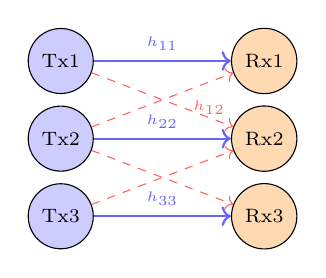
\begin{tikzpicture}[scale=0.68,
                    tx/.style={draw, circle, fill=blue!20, minimum size=0.62cm, font=\scriptsize},
                    rx/.style={draw, circle, fill=orange!30, minimum size=0.62cm, font=\scriptsize}]
                \foreach \i/\y in {1/1.45, 2/0, 3/-1.45}{
                        \node[tx] (tx\i) at (0, \y) {Tx\i};
                        \node[rx] (rx\i) at (3.8, \y) {Rx\i};
                        \draw[->, thick, blue!60] (tx\i) -- (rx\i)
                        node[midway, above, font=\tiny] {$h_{\i\i}$};
                    }
                \draw[->, dashed, red!60, thin] (tx1) -- (rx2)
                node[pos=0.65, right, font=\tiny] {$h_{12}$};
                \draw[->, dashed, red!60, thin] (tx2) -- (rx1);
                \draw[->, dashed, red!60, thin] (tx2) -- (rx3);
                \draw[->, dashed, red!60, thin] (tx3) -- (rx2);
            \end{tikzpicture}

            \vspace{0.1em}
            {\scriptsize \textcolor{blue!60}{---} desired \;
                \textcolor{red!60}{- -} interference}
        \end{column}
    \end{columns}
\end{frame}

% ----------------------------------------------------------------
% 3. RIBBO Method
% ----------------------------------------------------------------
\section{Method}

\begin{frame}{RIBBO: In-Context Black-Box Optimization}
    \small
    \footerref{Song et al., ``RIBBO: Reinforce Learned Black-Box Optimization with In-Context Learning,'' IJCAI 2025.}

    \begin{columns}[T,onlytextwidth]
        \begin{column}{0.47\textwidth}
            \textbf{Core idea}
            \begin{tightitemize}
                \item Learn a BBO \emph{algorithm} (not a solution)
                \item Input: history $(\mathbf{x}_{1:t},\,y_{1:t},\,R_{1:t})$
                \item Output: next query $\hat{\mathbf{x}}_{t+1}$
                \item Backbone: Causal Transformer (GPT-2)
            \end{tightitemize}
        \end{column}
        \begin{column}{0.49\textwidth}
            \textbf{Key ingredients}
            \begin{tightitemize}
                \item \textbf{RTG} (Regret-To-Go): conditions model on remaining improvement budget
                \item \textbf{HRR} (Hindsight Regret Relabelling): relabels any offline trajectory as near-optimal
                \item \textbf{Data:} $K$ algorithms $\times$ $N$ tasks $\times$ $T$ steps
            \end{tightitemize}
        \end{column}
    \end{columns}

    \vspace{0.7em}
    \centering
    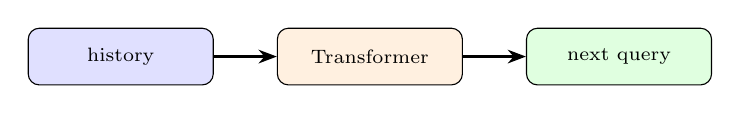
\begin{tikzpicture}[
            node distance=0.45cm and 0.8cm,
            box/.style={draw, rounded corners, fill=gray!10,
                    minimum width=2.35cm, minimum height=0.72cm,
                    align=center, font=\scriptsize},
            arr/.style={->, thick, >=Stealth}]
        \node[box, fill=blue!12] (hist) {history};
        \node[box, fill=orange!12, right=of hist] (tfm) {Transformer};
        \node[box, fill=green!12, right=of tfm] (query) {next query};
        \draw[arr] (hist) -- (tfm);
        \draw[arr] (tfm) -- (query);
    \end{tikzpicture}
\end{frame}

% ----------------------------------------------------------------
% 4. Pipeline
% ----------------------------------------------------------------
\section{Implementation}

\begin{frame}{Implementation Pipeline}
    \small
    \centering
    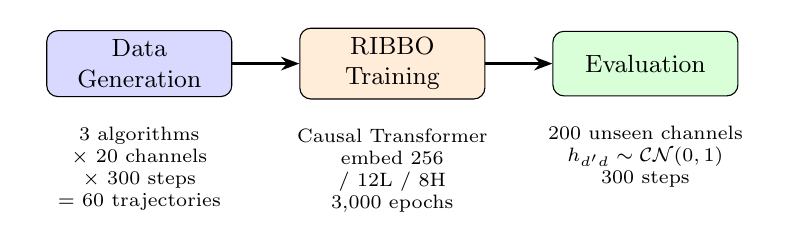
\begin{tikzpicture}[
            node distance=0.45cm and 0.85cm,
            box/.style={draw, rounded corners, fill=gray!10,
                    minimum width=2.35cm, minimum height=0.82cm,
                    align=center, font=\small},
            arr/.style={->, thick, >=Stealth}]

        \node[box, fill=blue!15]   (dg) {Data\\Generation};
        \node[box, fill=orange!15, right=of dg] (tr) {RIBBO\\Training};
        \node[box, fill=green!15,  right=of tr] (ev) {Evaluation};

        \draw[arr] (dg) -- (tr);
        \draw[arr] (tr) -- (ev);

        \node[below=0.25cm of dg, align=center, font=\scriptsize, text width=2.6cm]
        {3 algorithms\\$\times$ 20 channels\\$\times$ 300 steps\\= 60 trajectories};

        \node[below=0.25cm of tr, align=center, font=\scriptsize, text width=2.65cm]
        {Causal Transformer\\embed 256 / 12L / 8H\\3{,}000 epochs};

        \node[below=0.25cm of ev, align=center, font=\scriptsize, text width=2.65cm]
        {200 unseen channels\\$h_{d'd}\!\sim\!\mathcal{CN}(0,1)$\\300 steps};
    \end{tikzpicture}

    \vspace{0.55em}
    \begin{columns}[T,onlytextwidth]
        \begin{column}{0.47\textwidth}
            \raggedright
            \textbf{Behavior algorithms (data gen)}
            \begin{tightitemize}
                \item Random Search
                \item Hill Climbing
                \item CMA-ES
            \end{tightitemize}
        \end{column}
        \begin{column}{0.49\textwidth}
            \raggedright
            \textbf{Key implementation}
            \begin{tightitemize}
                \item \texttt{IFCMetaProblem}: IFC task class added to RIBBO codebase
                \item Per-channel RTG normalization
                \item Checkpoint resume across training sessions
            \end{tightitemize}
        \end{column}
    \end{columns}
\end{frame}

% ----------------------------------------------------------------
% 5. Convergence Check (Rastrigin)
% ----------------------------------------------------------------
\section{Results}

\begin{frame}{Convergence Verification --- BBOB Rastrigin}
    \small
    \begin{columns}[T,onlytextwidth]
        \begin{column}{0.42\textwidth}
            \textbf{Setup}
            \begin{tightitemize}
                \item Problem: Rastrigin (dim=10, BBOB)
                \item 20 tasks $\times$ 3 algorithms $\times$ 300 steps
                \item 1{,}000 epochs, RTX 4070 Ti ($\approx$51 min)
            \end{tightitemize}

            \vspace{0.3em}
            \textbf{Result}
            \begin{tightitemize}
                \item x-loss (Gaussian NLL): converges by epoch $\approx$600
                \item Early oscillation due to LR warmup (10k steps)
                \item Epoch 1: $+10.8$ \;$\to$\; Epoch 1000: $-44.9$
            \end{tightitemize}
        \end{column}
        \begin{column}{0.54\textwidth}
            \centering
            \vspace{-0.3em}
            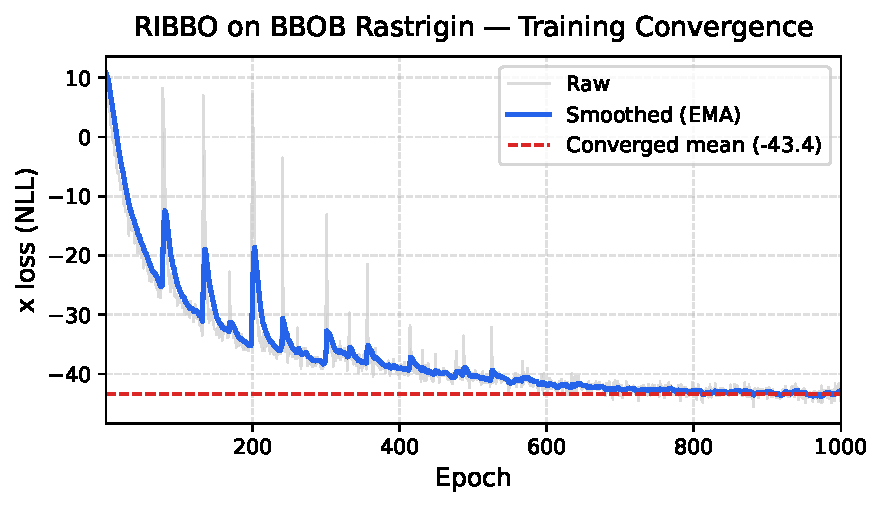
\includegraphics[width=\linewidth,height=0.56\textheight,keepaspectratio]{convergence_rastrigin.pdf}
        \end{column}
    \end{columns}
\end{frame}

% ----------------------------------------------------------------
% 6. IFC Training Convergence
% ----------------------------------------------------------------
\begin{frame}{IFC SE Training Convergence --- 3{,}000 Epochs}
    \small
    \begin{columns}[T,onlytextwidth]
        \begin{column}{0.42\textwidth}
            \textbf{Setup}
            \begin{tightitemize}
                \item 20 train channels $\times$ 3 algorithms $\times$ 300 steps
                \item embed 256 / 12 layers / 8 heads
                \item RTX 4070 Ti, $\approx$2.5 h
            \end{tightitemize}

            \vspace{0.3em}
            \textbf{Result}
            \begin{tightitemize}
                \item Epoch 1: $+2.9$ \;$\to$\; Epoch 3000: $-18.6$
                \item Oscillation larger than Rastrigin\\
                (channel-specific reward scale)
                \item Stabilizes by epoch $\approx$2{,}500
            \end{tightitemize}
        \end{column}
        \begin{column}{0.54\textwidth}
            \centering
            \vspace{-0.3em}
            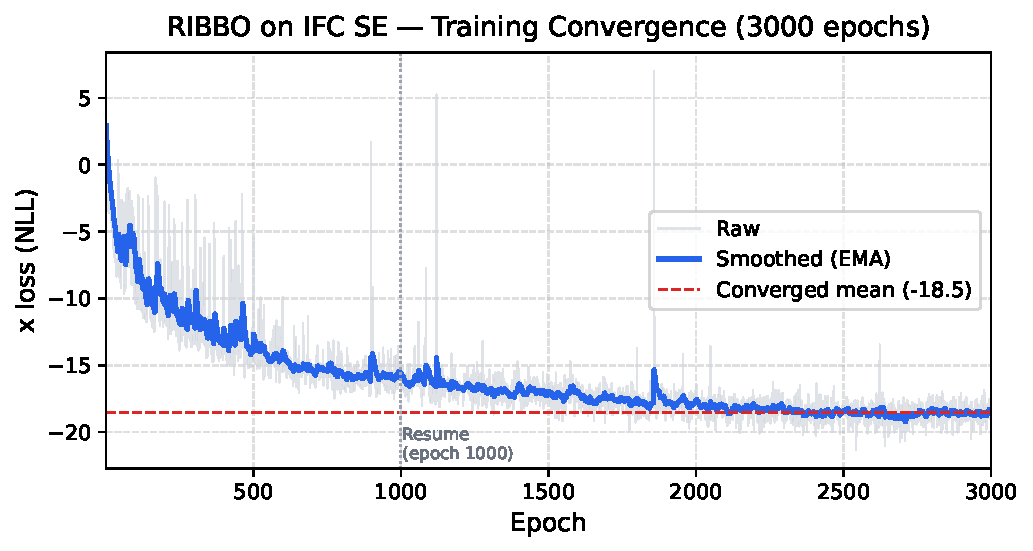
\includegraphics[width=\linewidth,height=0.56\textheight,keepaspectratio]{convergence_ifc.pdf}
        \end{column}
    \end{columns}
\end{frame}

% ----------------------------------------------------------------
% 7. IFC Evaluation Results
% ----------------------------------------------------------------
\begin{frame}{IFC SE Evaluation --- RIBBO vs.\ Random}
    \small
    \begin{columns}[T,onlytextwidth]
        \begin{column}{0.42\textwidth}
            \textbf{Evaluation setup}
            \begin{tightitemize}
                \item 200 unseen channels, $h_{d'd}\!\sim\!\mathcal{CN}(0,1)$
                \item 300 steps (in-distribution)
                \item Metric: best $r_{\mathrm{SE}}$ found so far (avg over channels)
            \end{tightitemize}

            \vspace{0.3em}
            \textbf{Final result @ step 300}
            \par\vspace{0.2em}
            \scriptsize
            \begin{tabular}{lrr}
                \toprule
                Method       & nats          & bits          \\
                \midrule
                RIBBO (ours) & \textbf{2.67} & \textbf{3.85} \\
                Random       & 2.44          & 3.52          \\
                \bottomrule
            \end{tabular}

            \vspace{0.3em}
            \small RIBBO $+$9.5\% over random baseline
        \end{column}
        \begin{column}{0.54\textwidth}
            \centering
            \vspace{-0.3em}
            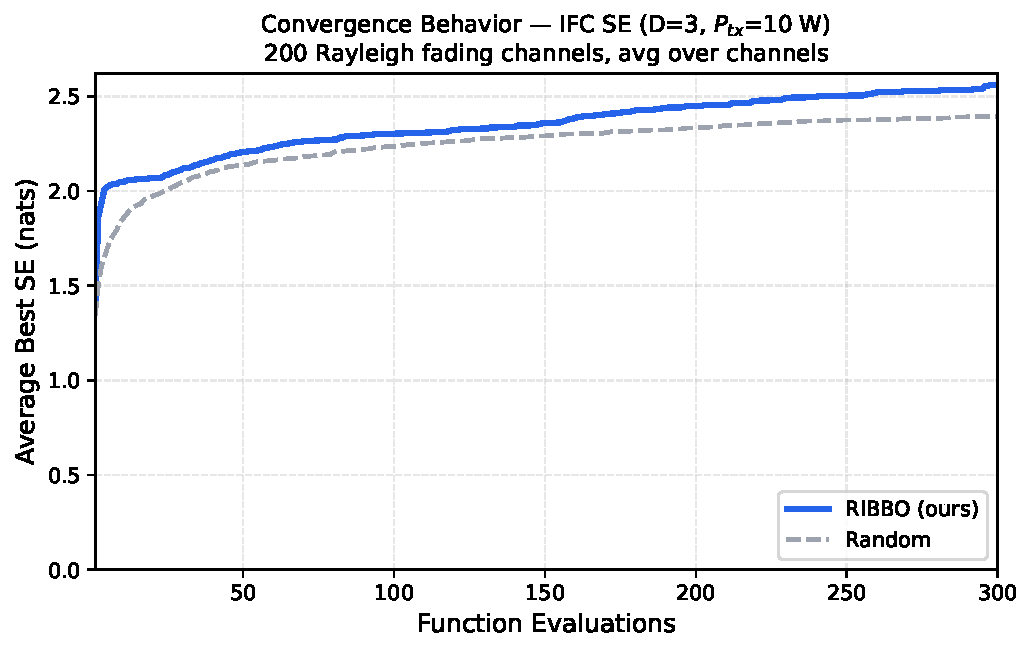
\includegraphics[width=\linewidth,height=0.56\textheight,keepaspectratio]{eval_ifc_matched.pdf}
        \end{column}
    \end{columns}
\end{frame}

% ----------------------------------------------------------------
% 8. Summary
% ----------------------------------------------------------------
\begin{frame}{Summary}
    \small
    \begin{columns}[T,onlytextwidth]
        \begin{column}{0.48\textwidth}
            \textbf{Completed}
            \begin{tightitemize}
                \item[\checkmark] IFC SE task integrated into RIBBO codebase
                \item[\checkmark] 60 offline trajectories generated \\(3 algos $\times$ 20 channels)
                \item[\checkmark] Training converged: 3{,}000 epochs
                \item[\checkmark] RIBBO outperforms random on 200 unseen channels
            \end{tightitemize}
        \end{column}
        \begin{column}{0.48\textwidth}
            \textbf{Next steps}
            \begin{tightitemize}
                \item Compare against CMA-ES baseline (strongest behavior algo)
                \item Extend trajectory length to 500 steps for direct comparison with Lee et al.
                \item EE reward variant
            \end{tightitemize}
        \end{column}
    \end{columns}
\end{frame}

\end{document}
